%!TEX TS-program = xelatex  
%!TEX encoding = UTF-8 Unicode  
\documentclass[11pt,a4paper]{paper}
\usepackage{float}
\usepackage{indentfirst}
\usepackage{geometry} 
\usepackage{enumitem} 
\usepackage{amsmath}      
\usepackage{fontspec,xltxtra,xunicode}  

\usepackage[]{xeCJK}
\XeTeXlinebreaklocale “zh”  
\XeTeXlinebreakskip = 0pt plus 1pt minus 0.1pt 

\author{Steven Shen \quad \quad}
\title{Proposal}

\begin{document}
\maketitle

\section{Statement of the Problem}

\textbf{Is the CO2?} 


\begin{figure}[!htb]
\centering
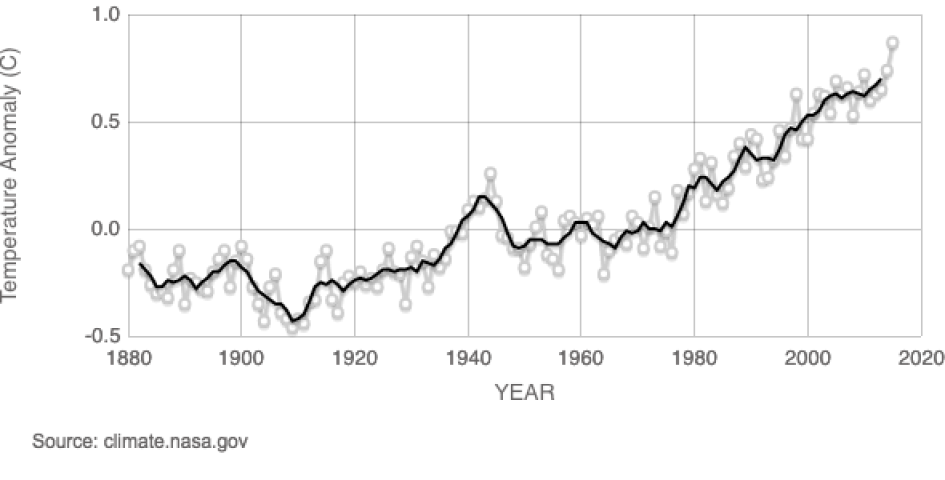
\includegraphics[scale=.30]{pic2.png}
\end{figure}

\begin{figure}[!htb]
\centering
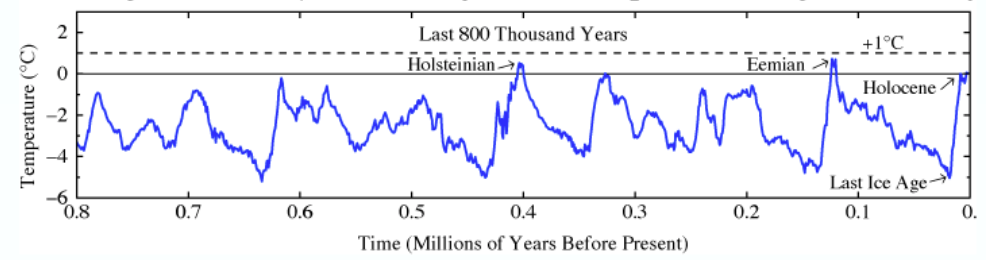
\includegraphics[scale=.40]{pic1.png}
\end{figure}

\section{Review of Previous Work}
There has been ferocious dabates on this problem. The major two are the `warmer' and the `lukewarmer'.


Supporters of the `warmer’ and `lukewarmer’ views tend to favour different global temperature datasets, which show different temperature trends in recent years.  A favourite of the warmers is NASA’s GISS data, whose land-ocean version combines land temperature observations with sea surface temperature data. This data set was recently revised, with the new version showing a larger upward trend in temperature in recent years. The lukewarmers tend to favour the UAH data from satellite observations, also recently revised, with the new version showing a lower trend than before.





\section{Description of Data}
see ``./data/log.txt``

\end{document}